\documentclass{article}
\usepackage[utf8]{inputenc}
\usepackage{multicol}
\usepackage{multirow}
\usepackage{authblk}
\usepackage{graphicx}
\newcommand\myfigure[1]{%
\medskip\noindent\begin{minipage}{\columnwidth}
\centering%
#1%
\end{minipage}\medskip}
\usepackage{amsmath}
\usepackage{hyperref}
\usepackage{subcaption}
\usepackage{adjustbox}
\usepackage{biblatex}
\usepackage{hyperref}
\hypersetup{
    colorlinks=true,
    linkcolor= violet,
    filecolor=magenta,      
    urlcolor=teal,
    citecolor = cyan,
    }

\urlstyle{same}
\usepackage{xcolor}
\usepackage{algpseudocode}
\usepackage{algorithm}

\title{\textbf{Fast Point Cloud Sampling Network}}
\author[a]{\textbf{Tianxin Huang}}
\author[a,\footnote{Corresponding author}]{\textbf{Yong Liu}}
\author[a,b]{\textbf{Jie Liang}}
\affil[a]{\textit{\small{Laboratory of Advanced Perception on Robotics and Intelligent Learning, College of Control Science and Engineering, Zhejiang University, Hangzhou, China}}}
\affil[b]{\textit{\small{Beijing Institute of Mechanical and Electrical Engineering, Beijing, China}}}
\date{}

\addbibresource{biblio.bib}
\begin{document}
\maketitle

\begin{abstract}
The increasing number of points in 3D point clouds has brought great challenges for subsequent algorithm efficiencies. Down-sampling algorithms are adopted to simplify the data and accelerate the computation.
\end{abstract}

\begin{multicols}{2}
\section{Introduction}
Existing works \cite{Pointnet} - \cite{DeepHough} often use random sampling and the farthest point sampling(FPS) to down-sample the point clouds.\par
The differences between our work and former learning-based works are presented in \textcolor{violet}{Fig} \ref{figure 1}.
\par
The discrepancy between progress-net and our method is
presented in \textcolor{violet}{Fig} \ref{fig:second}\textcolor{violet}{(b)} and 
\ref{fig:third}\textcolor{violet}{(c)}.\par

\begin{figure}
    \centering
    \caption{}
    \label{fig:my_label}
\end{figure}

\myfigure{
\begin{subfigure}{\columnwidth}
    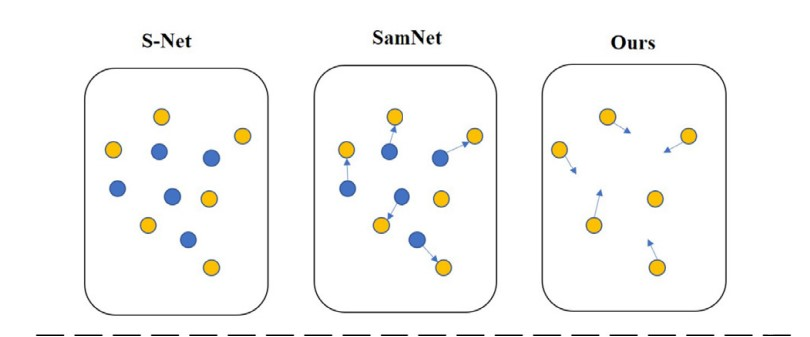
\includegraphics[width=\textwidth]{1a.jpg}
    \caption{(a)}
    \label{fig:first}
\end{subfigure}
\hfill
\begin{subfigure}{\columnwidth}
    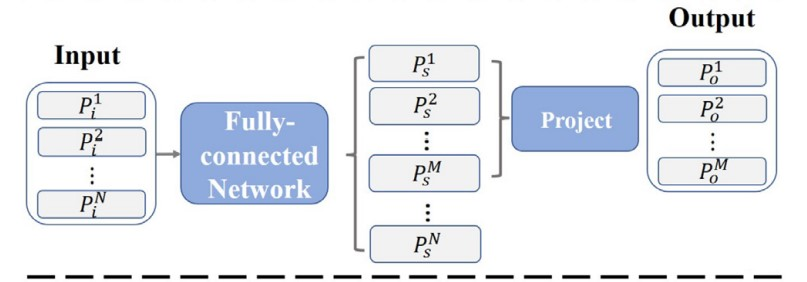
\includegraphics[width=\textwidth]{1b.jpg}
    \caption{(b)}
    \label{fig:second}
\end{subfigure}
\hfill
\begin{subfigure}{\columnwidth}
    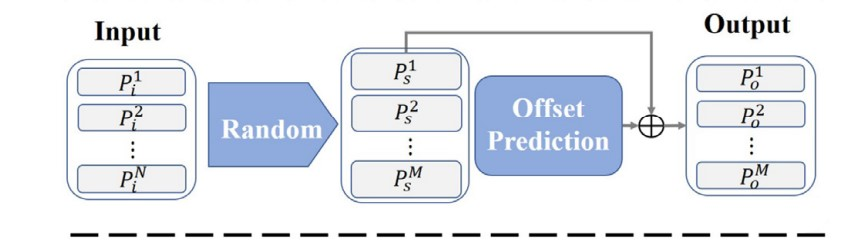
\includegraphics[width=\textwidth]{1c.jpg}
    \caption{(c)}
    \label{fig:third}
\end{subfigure}
\hfill
\figcaption {Figure 1:(a) shows the differences between
learning-based sampling strategies, while (b) and (c) present
the discrepancy between progress-net and our method in 
multiresolution sampling}
\label{figure 1}
}

\par
Our contributions can be summarized as:
\begin{itemize}
    \item  We propose a novel learning-based point cloud 
    sampling framework named fast sampling network (FPN) by 
    driving existing randomly sampled points to better 
    positions;

    \item We introduce a hybrid training strategy to help FPN 
    adapt to different sampling resolutions by randomly 
    introducing selecting the resolution of initial points 
    during training;\par
\end{itemize}

\section{Methodology}
\subsection{\textit{Basic pipeline}}
The basic pipeline of FPN is presented in \textcolor{violet}{Fig} \ref{figure 2} We aggregate global features from the input points with a set of multilevel perceptions (MLPs) and Max Pooling following PointNet \cite{PointNet2}.\par
The achievement of HTS is presented as \textcolor{violet}{Algorithm} \ref{Algo 1}.

\subsection{\textit{Loss fuction}}
The range constraint can be presented as

\begin{equation}
    L_{rc} = \frac{1}{N} \sum ||S_o - S_i||_2,
\end{equation}

For reconstruction related tasks, it may be Chamfer Distance or Earth Mover Distance \cite{KPConv} defined as

\begin{equation}
\begin{split}
    L_{task} & = L_{CD}(S_1,S_2) \\
             & = \frac{1}{2} (\frac{1}{|S_1|}\sum_{x \in S_1} \min_{y \in S_2} ||x-y||_2 + \frac{1}{|S_2|}\sum_{x \in S_2} \min_{y \in S_1} ||x-y||_2),
\end{split}
\end{equation}  

or

\begin{equation}
    L_{task} = L_{EMD}(S_1,S_2) = \min_{\phi:S_1\xrightarrow{}S_2}\frac{1}{|S_1|}\sum_{x \in S_1} ||x-\phi(x)||_2,
\end{equation}

where $S_1$ and $S_2$ are input and output. $\phi$ is a bijection from $S_1$ to $S_2$.

\section{Experiments}
\subsection{\textit{Dataset and implementation details}}
\textbf{Table 1} \par
The number of neurons in networks. $f_1$ , $f_2$ , $f_3$ are modules in \textcolor{violet}{Fig} \ref{figure 2}.\par

\scalebox{0.75}{
\begin{minipage}{0.7\linewidth}
\begin{tabular}{c c c c}
\hline
& $f_1$ & $f_2$ & $f_3$ \\
\hline
MLPs & (128,256,256) & (128,256,256) & (128,128,3)\\
\hline
\label{Table 1}
\end{tabular}
\end{minipage}%
}
\\
\\
\textbf{Table 2} \par
The comparison on optimal clustering.

\begin{tabular}{ c c c c c}
\hline
Center & iterations & 1 & 10 & 100 \\ 
\hline
\multirow{2}{*}{16} & FPS  & 2.43 & 2.00 & 1.98 \\
 & Ours & \textbf{2.16} & \textbf{1.98}  & \textbf{1.96} \\
 \multirow{2}{*}{32} & FPS  & 1.20 & 1.02 & 1.00 \\
 & Ours & \textbf{1.11} & \textbf{1.00} & \textbf{1.00}\\
 \hline
 \label{Table 2}
\end{tabular}

The hyper-parameter $\lambda$ is tuned on the validation split of ShapeNet. Detailed network structures are shown in \textcolor{violet}{Table} \ref{Table 1}.

\end{multicols}

\begin{figure}
    \centering
    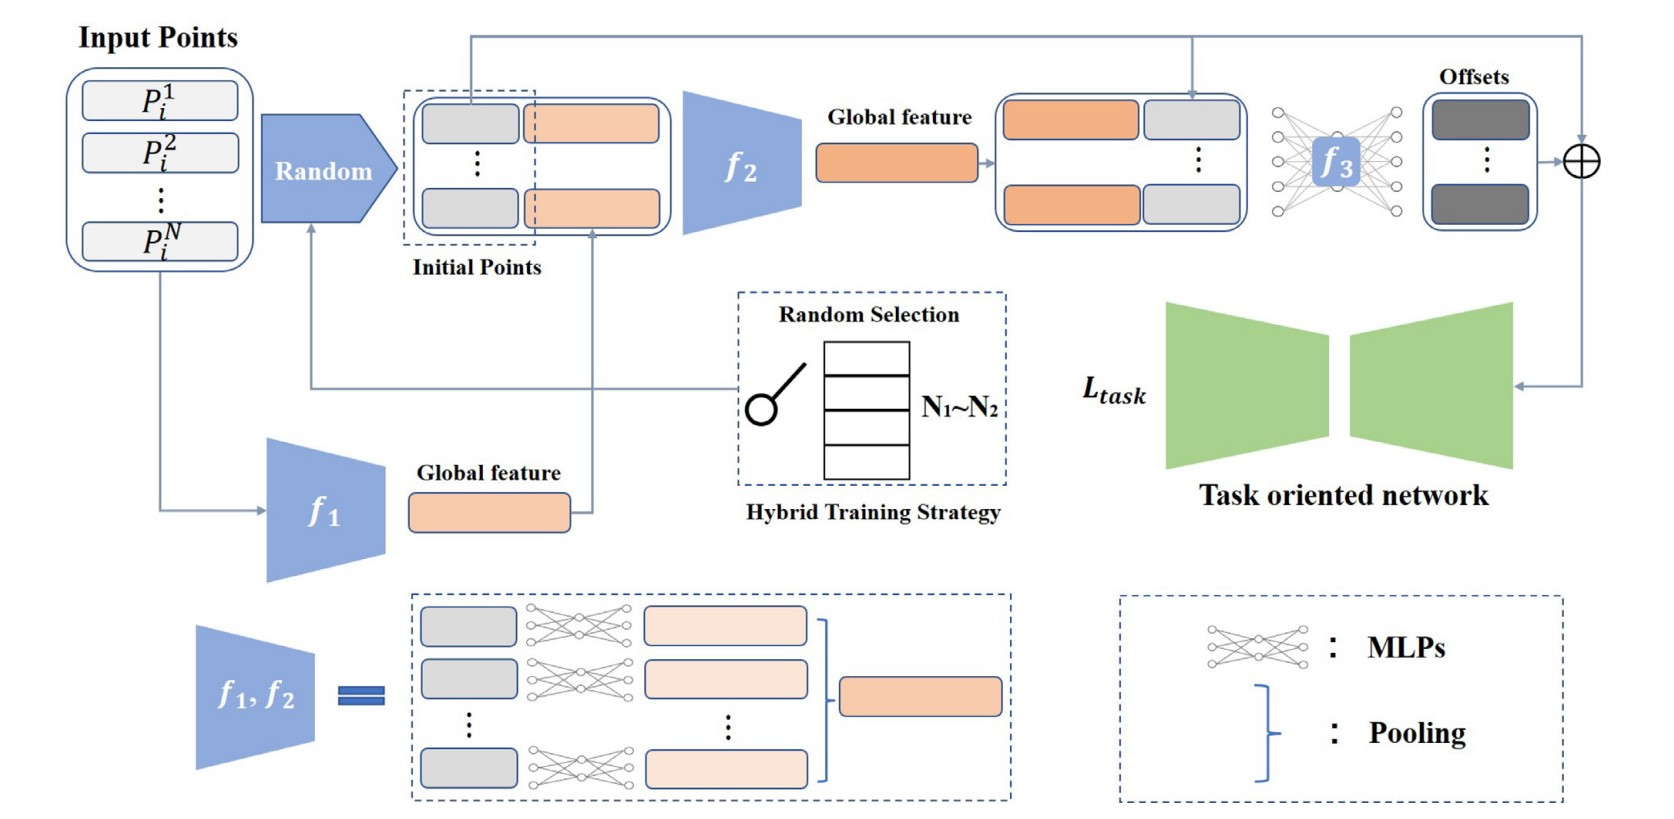
\includegraphics[width = 0.8\textwidth]{2.jpg}
    \caption{The whole pipeline of FPN. The + denotes element-wised addition. $f_1$ and $f_2$ aggregate features by MultiLayer Perceptrons(MLPs) and pooling, while $f_3$ is a group of MLPs to predict offsets from coordinates and features. The task network is corresponding to the specific task, such as point cloud recognition and reconstruction. $L_{task}$ is the loss constrained the task network}
    \label{figure 2}
\end{figure}

\newpage
\begin{multicols}{2}
\subsection{\textit{Discussion about clustering}}\label{Section}
Except down-stream tasks such as reconstruction or recognition, down-sampled points can also be adopted as the initial clustering centers. \cite{Clustering} \par
The results are presented in \textcolor{violet}{Table} \ref{Table 2}.

\subsection{\textit{Ablation study}}
\textbf{The influence of range constraint.} Note that this is only conducted to observe the influence of range constraint weight $\lambda$ on sampling performances instead of the tuning of $\lambda$, which is chosen according to the val set
introduced in \textcolor{violet}{Section} \ref{Section}.\par

\scalebox{1}{
\begin{minipage}{\linewidth}
\begin{algorithm}[H]
\caption{ Training with Hybrid Training Strategy}
\begin{algorithmic}
\State \textbf{Input: } data $X$ the number of iterations $iter$, the number of resolutions $m$;
\State $prob_1$,$prob_2$,\dots,$prob_m$ 
\State = $\frac{1}{m}$,$\frac{1}{m}$,\dots,$\frac{1}{m}$;
\For {$i=1$ to $iter$}
    \State Select the resolution $r$ according to $prob_1$,\dots,$prob_m$;
    \State Train FPN by descending gradient: $\delta_{\theta_{FPN}}L_{loss}(Y_{X,r})$
\EndFor
\end{algorithmic}
\label{Algo 1}
\end{algorithm}
\end{minipage}%
}

\section*{\textbf{Data availability}}
Data will be made available on request
\section*{\textbf{Acknowledgement}}
We thank all reviewers and the editor for excellent contributions. This work is supported by the Key Research and Development Project of Zhejiang Province under Grant 2021C01035.
\end{multicols}


\printbibliography

\end{document}
